% --------------------------------------------------------------
% This is all preamble stuff that you don't have to worry about.
% Head down to where it says "Start here"
% --------------------------------------------------------------
 
\documentclass[12pt]{article}

\renewcommand{\thesubsection}{\thesection.\alph{subsection}}
\usepackage{todonotes}
\usepackage[margin=2cm]{geometry} 
\usepackage[backend=bibtex]{biblatex}
\addbibresource{ref.bib}
\usepackage[]{quoting}
\usepackage{listings}[language=C]
\usepackage{xcolor}
\usepackage{float}


\definecolor{codegreen}{rgb}{0,0.6,0}
\definecolor{codegray}{rgb}{0.5,0.5,0.5}
\definecolor{codered}{rgb}{0.64, 0.03, 0.22}
\definecolor{backcolour}{rgb}{0.9,0.9,0.9}

\lstdefinestyle{mystyle}{
    backgroundcolor=\color{backcolour},   
    commentstyle=\color{codered},
    keywordstyle=\color{magenta},
    numerstyle=\tiny\color{codegray},
    stringstyle=\color{codered},
    basicstyle=\ttfamily\footnotesize,
    breakatwhitespace=false,         
    breaklines=true,                 
    captionpos=b,                    
    keepspaces=true,                 
    numbers=left,                    
    numbersep=5pt,                  
    showspaces=false,                
    showstringspaces=false,
    showtabs=false,                  
    tabsize=2
}

%\lstset{style=mystyle}

\usepackage{amsmath,amsthm,amssymb}
\usepackage[english]{babel} %Castellanización
\usepackage[T1]{fontenc} %escribe lo del teclado
\usepackage[utf8]{inputenc} %Reconoce algunos símbolos
\usepackage{lmodern} %optimiza algunas fuentes
\usepackage{graphicx}
\graphicspath{ {images/} }
\usepackage{hyperref} % Uso de links
 \hypersetup{
  colorlinks=true,
  linkcolor=blue!50!red
}

\begin{document}
 
% --------------------------------------------------------------
%                         Start here
% --------------------------------------------------------------
 
\title{MiniTwit Report \\
DevOps \\
BSDSESM1KU \\
(Data Science)}

\author{Anders Stendevald (andst@itu.dk) \\ 
Anna Reisz, (reis@itu.dk) \\ 
Edi Begovic (edbe@itu.dk) \\ 
Gergo Koncz (geko@itu.dk) \\ 
Høgni Jacobsen (hoja@itu.dk)\\
}

\maketitle
\clearpage
\section{Introduction}
MiniTwit is a Twitter clone originally written by ITU researchers. Since then, the web application have been neglected, with no maintenance being done. This changed in 2021. In the name of DevOps a handful of students decided to update it. 
\\\\
The following sections will cover: the System's Perspective -including the choices for the technology used in the project, then the Process' perspective -including the way the team worked together and the how the decisions were made. The Lessons Learned Perspective includes our reflections on the project and the elements that we would have done differently.

\section{System's Perspective}
This section will cover the technology details of our system. Only the most significant elements will be covered. This includes our considerations when creating maintainable software. An explanation of the Minitwit application, and some of the most prominent technologies used in the project. Namely Docker, Django, the CI/CD and our static Code Analysis.   

\subsection{Creating maintainable software}
Before we cover the details of our project, we wish to stress the importance of a DevOps mindset. Code should never be static and should always be up to date. But as a developer with limited resources, you simply cannot be the only maintainer of an entire software stack. Therefore you should always strive to create software that can be given to new people without worry. This includes automating as many things as possible. At worst give new people an insight into how a piece of software should work. \\\\
This also means adopting a high standard of testing and adding doc strings to code. Ultimately a piece of software is only finished when the code runs, the tests pass and the documentation is clear. This is especially important in DevOps.
\\\\
One last note that was especially important for this project was the use of docker files for testing and deployments. When you create a DockerFile, you not only automate the build steps of the application. You also document the target platform and the dependencies. This comes almost entirely for free, which makes it even more valuable to adopt Docker. 

%\subsection{What we need to do}
%A description and illustration of the:
% \begin{itemize}
%     \item Design of your ITU-MiniTwit systems
%     \item Architecture of your ITU-MiniTwit systems
%     \item All dependencies of your ITU-MiniTwit systems on all levels of abstraction and development stages.
%     \item That is, list and briefly describe all technologies and tools you applied and depend on.
%     \item Important interactions of subsystems
%     \item Finally, describe the current state of your systems, for example using results of static analysis and quality assessment systems.
%     \item Double check that for all the weekly tasks (those in the end of the lecture notes) you include the corresponding information.

% \end{itemize}
\subsection{Application / architecture overview}
% \begin{itemize}
%     \item Design of your ITU-MiniTwit systems
%     \item Architecture of your ITU-MiniTwit systems
%     \item All dependencies of your ITU-MiniTwit systems on all levels of
% \end{itemize}

At the core of our application there are two Django apps interfacing with a single source-of-truth, a Postgres relational database. One of the Django apps is for the web frontend for regular users and the other is for the API to provide access for developers. The rest of the architecture surrounding the core is to enable the maintenance, development and evolution of the project in line with the devops mindset. Docker, docker-compose and docker swarm were utilized for virtualization and orchestration, Prometheus and grafana for monitoring and the ELK stack for logging. 
\begin{figure}[h!]
    \centering
    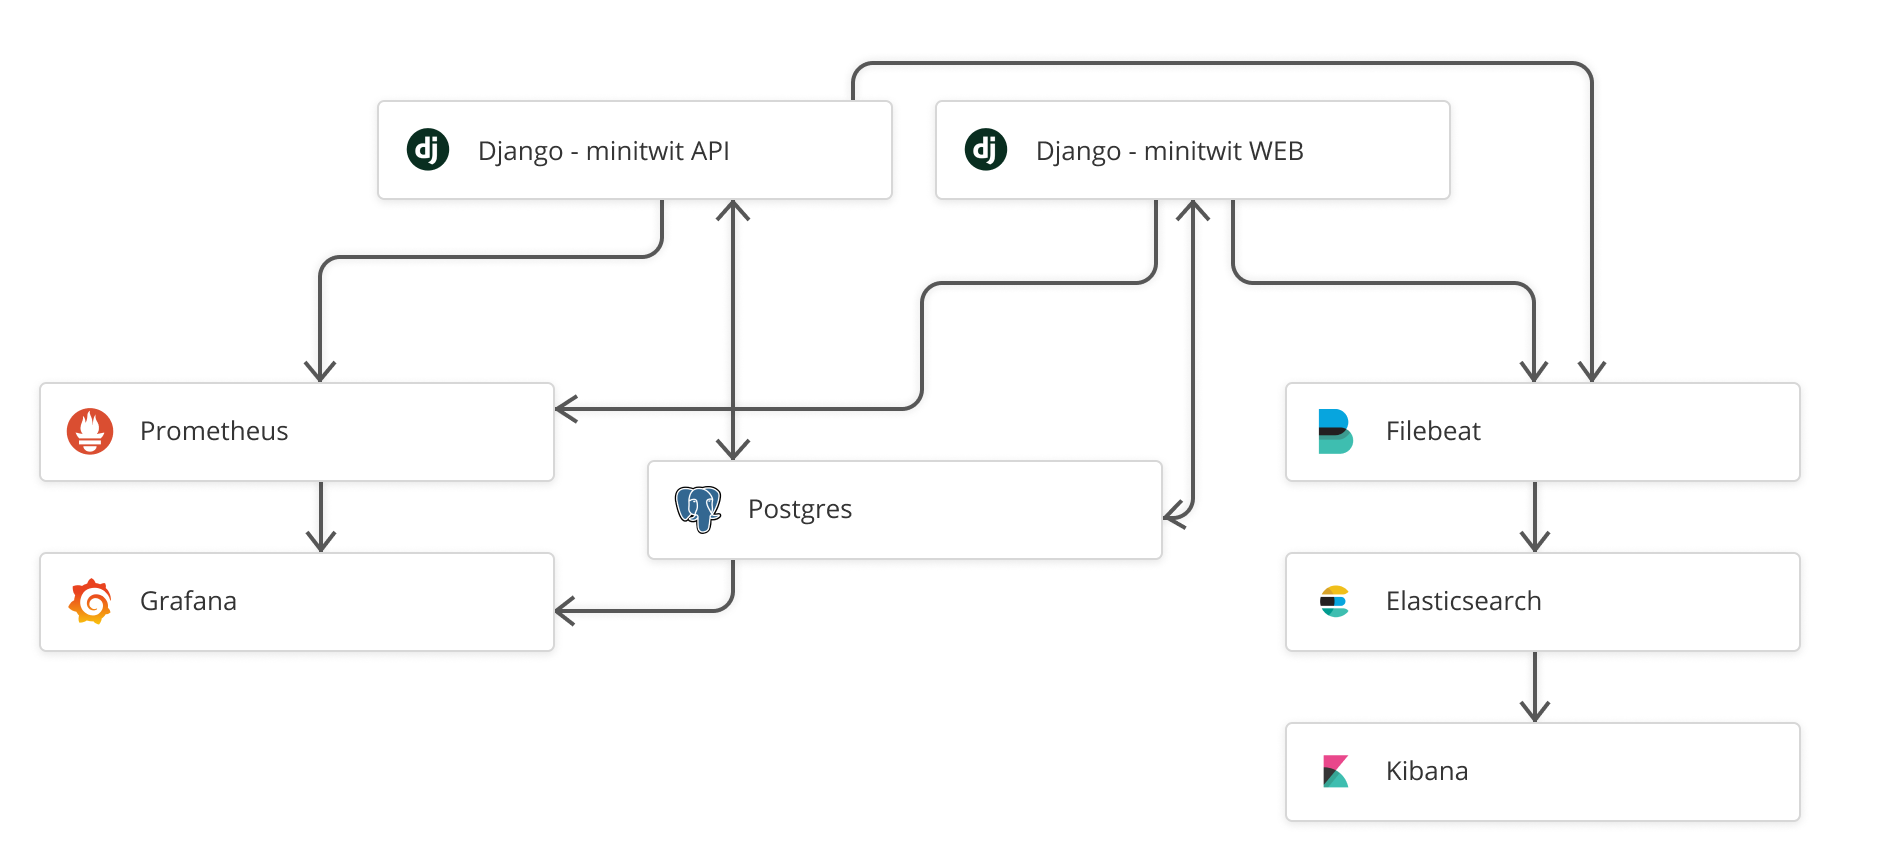
\includegraphics[width=8cm]{figures/structure}
    \caption{Application / architecture overview}
    \label{fig:structure}
\end{figure}

\subsection{Virtualisation}
It was essential for the project to utilize some sort of virtualisation. Not only would it make the application portable, but also make it run on any platform. Below we will discuss why we chose Docker for this instead of other approaches like Vagrant. 

\subsubsection{Docker}
At the core of Docker is the Open Container Initiative\footnote{\url{https://opencontainers.org/}}. This means that any docker images adheres to a spec determined by domain experts. This means that running an application with docker is not only cross compatible today, but also tomorrow. Even if another container orchestrate comes around. 
\\\\
In this project we decided to have every part of the project in its own container and image. This was without much overhead or extra developer time. The advantages were that the applications ran more secure, without elevated user rights. That the networking between containers were locked down. Making them more secure. All of this was orchestrated with docker compose. Making the DockerFiles simpler and more secure.   

\subsubsection{Not Vagrant}
The other option for a virtualisation stack was Vagrant. We opted not to go for this because our application consisted of many small sub components. Had we had a more complicated setup, with many connections between sub components. Then Vagrant would had been easier. It would also make it easier to deploy code to a fresh server. The overhead of developing on a Hypervisor would also not had been nice. For development docker is just easier. 
\subsection{Core Technology stack}

\subsubsection{Django}
\href{https://www.Djangoproject.com/}{Django} is a Python library for web development. We have chosen this because we all had experience with Python and Django is the de facto tool for full-stack python web development as it integrates well with the underlying database system and has multiple related tools that facilitate an ecosystem around web based applications unlike for example the Python based Flask. 

Both our web and API interface is built on Django. API orchestrates interaction with the database such as initial creation of tables, but both interacts with the database directly during production.

\subsubsection{Postgres}
\href{https://www.postgresql.org/}{PostgreSQL} is one of the most prevalent relational database systems. It is open source and has a nice integration with Django, therefore it was the straightforward choice to store relational data, it is also a tool that the team had as a skill. It is also faster than SQLite, the original database system.


\subsection{CI-CD pipeline}
We have decided to use GitHub actions to orchestrate continuous integration and development. We have found that this technology stack works inherently well with development using GitHub which speeds up development in general. (Trying to make it work with Travis or Jenkins for instance, involved connecting multiple technologies, which brought some unforeseen issues.) GitHub enforced a DevOps-thinking, that proved useful when we needed to integrate more technologies on top of our existing stack. For example we were able to use a marketplace action for pushing images to docker hub. Saving development time.

We have implemented two "actions". One functions as quality assurance. Every time we merge a fix-branch/feature branch into the development branch we run some test scripts and perform linting. This script also "deploys" our project to a "development server", set up as a clone of the production environment for testing without the risk failure or downtime on the real server (where the simulator was sending data).

The second "action" is used for deployment. In essence it works the same way, but it is triggered when we push code to the main branch and it deploys our code to the real server. This step also includes creating a new release.

\subsection{Linting}
For linting we used \href{https://github.com/psf/black}{Black} for Python. Helping us to keep coding styles concise, by automatically formatting code. Black is also run in the QA step in GitHub actions.

\subsection{Static Code Analysis}
We are using \href{https://xenon.readthedocs.io/en/stable/}{Xenon} for static code analysis. Xenon is a python tool that can asses code complexity. It is based on Radon, a tool that makes metrics based on the code's 
\href{https://radon.readthedocs.io/en/latest/intro.html}{cyclomatic complexity}. 

Xenon labels code files from A-F (A being the best), and our code have been passing grade B in \textit{block complexity, average complexity, modules complexity} -a threshold we have set for quality assessment, but our code right now passes grade A in modules complexity and average complexity.

\subsection{License}
After careful inspection of our dependencies' licenses we have decided to use GPL 3 license. This is largely because one of our dependencies have the same license which doesn't allow us to use a more open license such as MIT, which we would otherwise have preferred.


\section{Process' perspective}
The following section will cover the process elements of DevOps. This means the processes used to automate elements of development and the way the team, GitHub and communication was setup. When creating an optimal process it is important to adopt the right policies and ideas. Policies and ideas that makes the project easier to work with, easier to maintain and makes handover seamless. Both from the perspective of the Developer, but also the other stakeholders. When you adopt the right process, you end up having the right discussions, which is arguably the most important step in creating good software.

\subsection{Logging and monitoring of the application}
The addition of logging and monitoring for modern software is crucial in detecting and identifying the events occurring with the system. When proper logging is implemented it is quite easier to react to errors, exceptions happening. On one hand, with logging we can keep a tab of vast amount of events and with the help of the ELK stack all these events was transformed to be consumable. On the other hand, with monitoring we can zoom in on events in a more focused, maybe a bit more business-minded way and even create triggers for when outliers occur. It is especially important for when you handover an application. Logging makes it possible to show a newcomer how the application is used.
\\\\
To monitor the system we use database queries (Inside Grafana) and \href{https://github.com/giampaolo/psutil}{psutil} to pull system stats and pass them to Prometheus. We chose to monitor both business and technology related metrics. Below we cover the prominent technologies used in our logging and monitoring. All of them serve different purposes, but are all important.
\subsubsection{Prometheus}
\href{https://Prometheus.io/}{Prometheus} is a monitoring tool, which records events and metrics in a time-series database. We use Django-Prometheus, a library that integrates well with Django-based web applications. This monitors our Django-models (directly from the database), the health of the server (such as CPU load and memory usage), web traffic (such as http response codes) etc. We also use Prometheus\_client for monitoring additional metrics, however so far this was not necessary. 

\subsubsection{Grafana}
\href{https://grafana.com/}{Grafana} is an analytics visualization platform that can show dashboards of metrics provided by a monitoring tool such as Prometheus. Our dashboard  can be seen in \ref{fig:dash}. It is divided in two sections: one for technical purposes and one for business purposes. The technical part includes up-time, CPU load, memory usage and disk usage. This gives us an overview of whether maintenance is needed at a glance. The business part includes number of users, number posts and number of followers. This allows us to get a better overview of our product's popularity and makes us better understand how our users use the service.
\begin{figure}[h!]
    \centering
    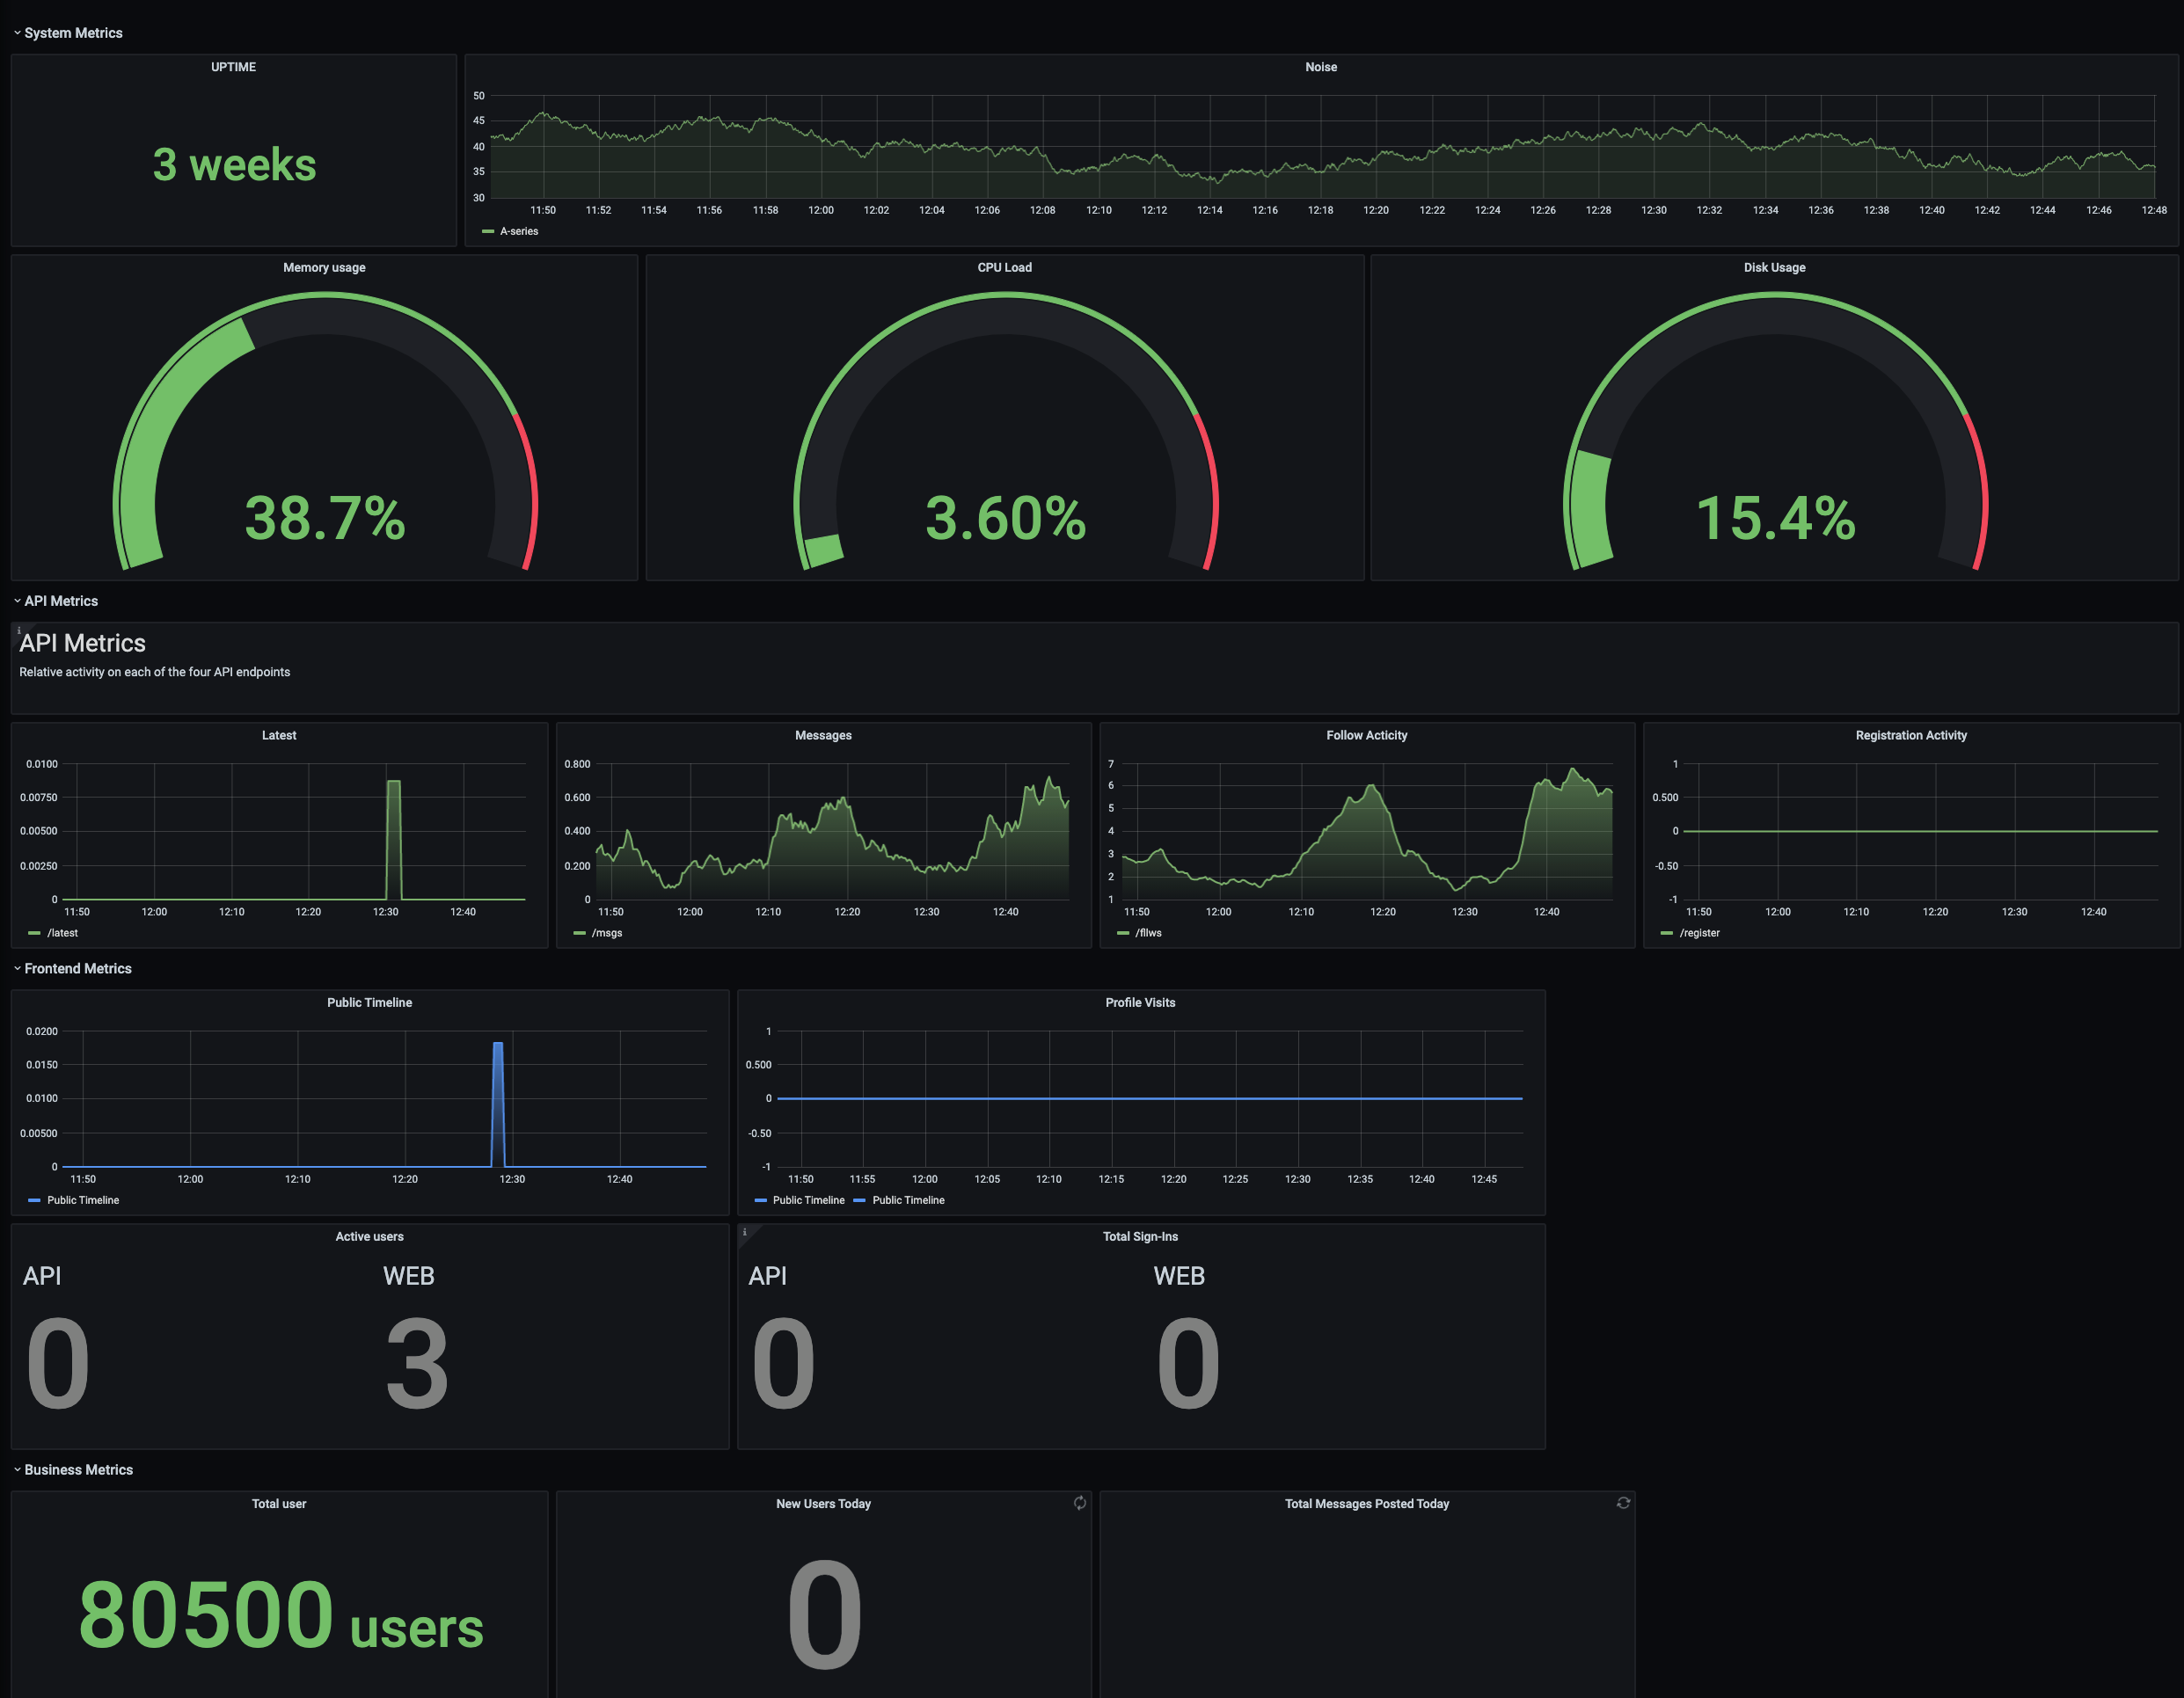
\includegraphics[width=12cm]{figures/Dash}
    \caption{Grafana dashboard}
    \label{fig:dash}
\end{figure}
\subsubsection{Filebeat}
\href{https://www.elastic.co/beats/filebeat}{Filebeat} is a lightweight shipper for logs. Its function is to collect and centralize logs from given locations on the server and forward them to the specified target, ElasticSearch in our case. Using a Filebeat container was quite seamless in our setup, the configuration is about specifying where the log files are dropped and in what form Filebeat should forward them. 

\subsubsection{Elasticsearch}
\href{https://www.elastic.co/elasticsearch/}{ElasticSearch} is a multipurpose RESTful search and analytics engine with its fast search as the core feature. It is part of the ELK stack and the software allows for several types of searches (structured, unstructured, geo, metric). We have used an ElasticSearch to collect and structure the logs collected by Filebeat and allow quick searching for the next tool in our logging pipeline.

\subsubsection{Kibana}
\href{https://www.elastic.co/kibana}{Kibana} is a flexible visualization tool that is the third element of the logging pipeline. Kibana transforms the logs structured by ElasticSearch into a more human-consumable format. Various visualizations can be utilized to make the logs more understandable and clearer.
\subsection{GitHub for collaboration}

As a developer team we mainly relied on having weekly meetings and discussing what product increments should be made. Afterwards we have been working on the new features in small teams or individually. To further improve on the organization of tasks we made use of GitHub issues, allowing for easy integration with the concrete implementation through pull requests.
\\\\
We were keen on keeping a team of equal voices, however if one of us had some previous experience with some of technologies we were to integrate into our app, that voice and the arguments with it carried naturally more weight. Also, in case a person wanted to delve into some solutions more or experiment with alternative solutions for given problem, it was encouraged. 
\\\\
We maintained two repositories one for the CI part of the pipeline and for the CD. In the repository for CI we have contained the application code and the parts necessary for local development. Furthermore GitHub actions for testing and building our Docker images, pushing them to the container registry. The deployment repository contained the configuration file needed for the deploying to the test and the production server.
\\\\
Working with development in git, we followed a strategy where the main branch was the bases of releases (first, weekly, later automatic releases). We avoided committing directly to the main branch, instead merging development into main via a pull request. We usually agreed on these merges at meeting as they had a major impact on the overall project. All features and fixes were developed on feature-branches which occasionally had sub-branches themselves when needed. Some of these sub-branches functioned as experiments and didn't lead anywhere, while others were merged back into the original feature branch which in turn was merged into the development branch as soon as the feature was complete. See Figure \ref{fig:branching}
\begin{figure}[h!]
    \centering
    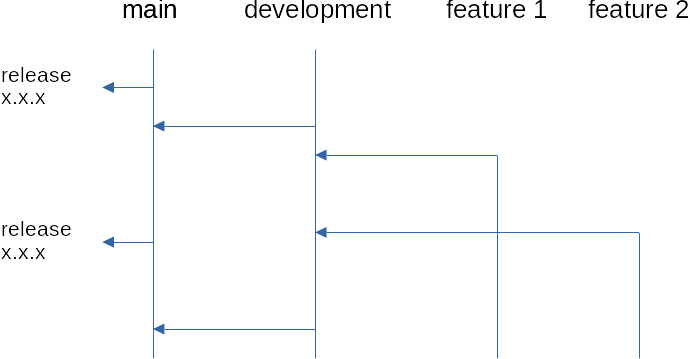
\includegraphics[width=12cm]{figures/branching.png}
    \caption{Branching strategy}
    \label{fig:branching}
\end{figure}
\subsection{Deployment and production CD}
Our deployment GitHub action started with installing requirements, then we tested our system both with scripts and static code analysis one last time, afterwards we built and pushed the images to docker hub, finally we deployed these images to our server /swarm using a freshly pulled docker-compose file from our deployment repository. This docker compose file made sure that we started the database first, then set up monitoring, then started our apps (Api, then Web), and finally set up logging. The CD process ended with creating a new release.
\\

\subsection{Handling traffic}
% Talk about the load balacing and the different steps. Floating IP, Swarm and Enigine X.
There are three layers to handling incoming traffic to our system. 
Firstly, we use a Digital Ocean floating IP which is a a flexible IP address that can be instantly mapped to any Digital Ocean service. A great advantage is the ability to experiment with different types of hardware without wait the 6-48 hours for the DNS to update the endpoint of our domain name. 
\ \\

\noindent
We use Docker Swarm to orchestrate the containers and allows us to seamlessly scale horizontally without having to manage “physical” machines or route traffic. A swarm consists of manager and worker nodes. Contrary to other distributed systems, the manager nodes don’t souly manage the incoming traffic. Instead, all nodes in the swarm are a part of a “routing mesh” which keeps track of which services run on all nodes. That way, incoming traffic to any node will automatically get routed to an instance of the service, even if it’s not running on the actual node. Thus, the routing mesh also acts as a simple load balancer, spreading request to the “least busy” instance of a service.

\begin{figure}[]
    \centering
    \makebox[\textwidth][c]{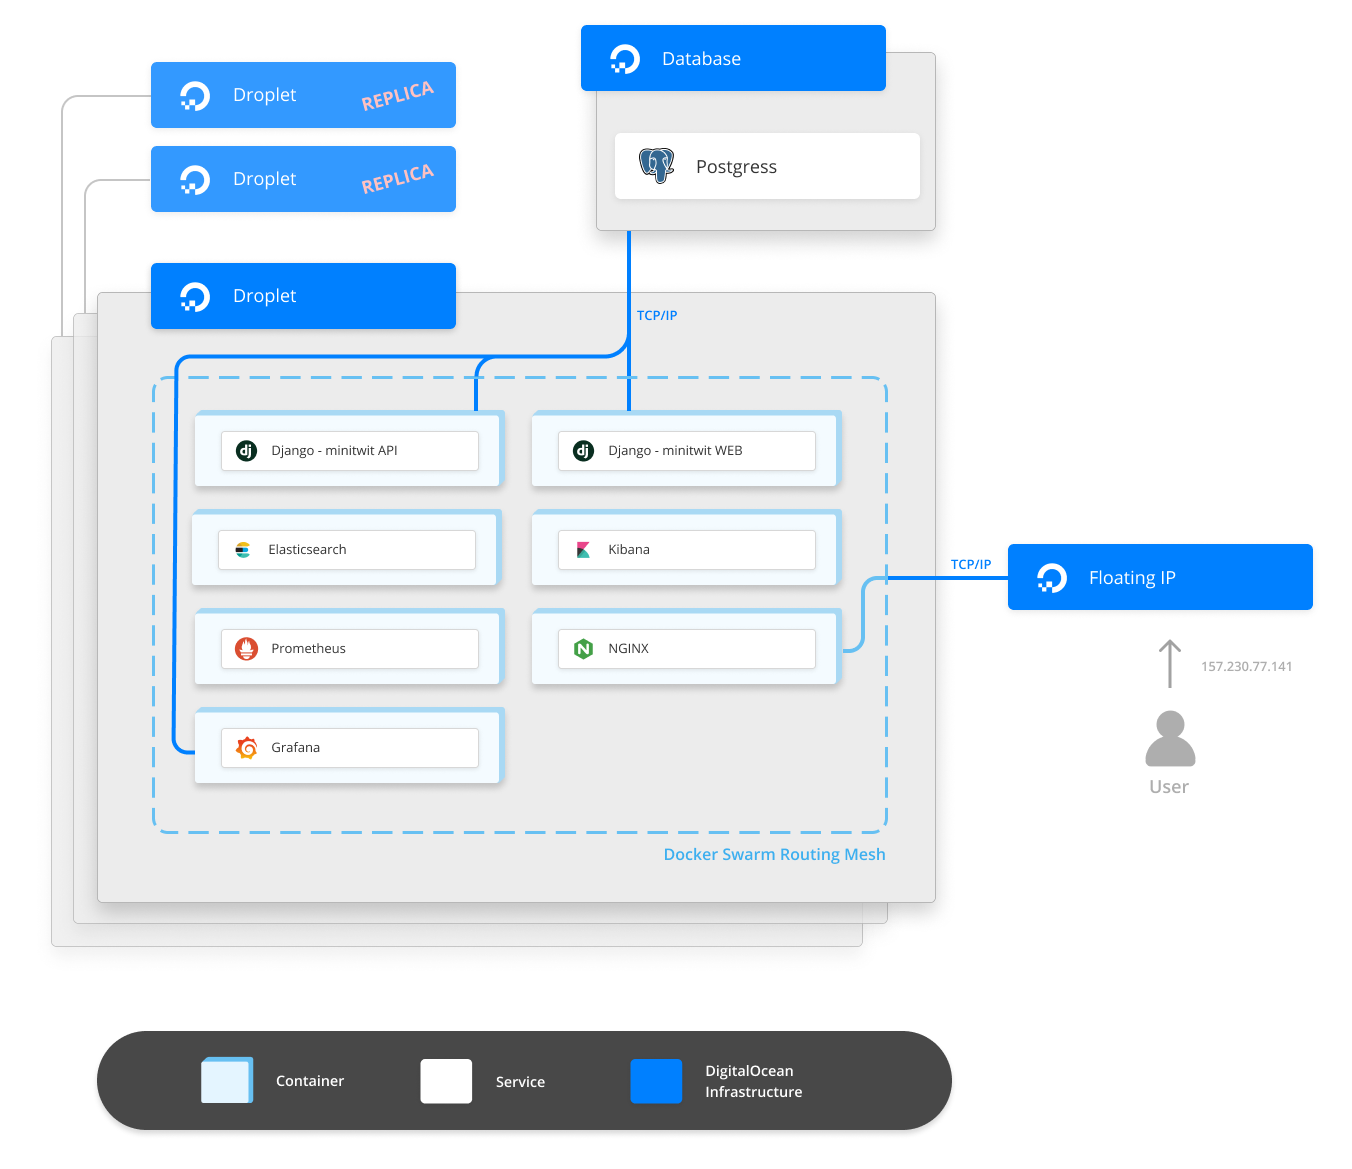
\includegraphics[width=1.2\textwidth]{figures/infrastructure}}
    \caption{Deployment overview}
    \label{fig:deployment_overview}
\end{figure}

% \\\\
% For example, how did you use issues, Kanban boards, etc. to organize open tasks
%     [GERGO]
    
% \\\\
\section{Lessons Learned Perspective}
This last section will conclude this DevOps project, by highlighting the lessons learned in the project. In an iterative process is a good thing to make mistakes. It is preferable from a learning perspective. This requires that mistakes are analysed and discussed. Otherwise a team might make the same mistake more than once. Even on different parts of the projects. In this section we highlight our venture into Kubernetes as a mistake. In this section we cover issues we had moving to Django, Kubernetes and its drawbacks, issues with the multi-App Django and security problems.
\subsection{Issues moving to Django}
The Old MiniTwit system was built on Python 2 and Flask. To migrate from Python 2 to 3 we used the Python module \textit{2to3}. This did not work perfectly and we had to manually change some code elements. Flask required some more work to migrate from. To migrate from Flask we had to get an overview of the system in Flask and then we could then build the Django application up section by section. We ran into some issues due to use having two team working on different parts of the refactoring. One working in the API the other on the web application. This issue was quickly fixed by a consultation and a decision as to how to continue.
\subsection{Kubernetes and its drawbacks}
During our final phases of development, we decided to adopt Kubernetes as our platform. We made this decision on the promise of rollover deployments, load balancing, centralised logging and horizontal scaling. This move seemed straight forward, especially after we had containerised the entire stack of the application and supporting layers. What we would gain is kind of the endgame of DevOps. Having infrastructure as code and deployments without having to rely on an SSH connection even for automated deployments. With all the promises of Kubernetes it might be confusing as to why we ended up not using Kubernetes in the end.
\\\\
While every component worked fine internally and individually, we had problems configuring the incoming connections and putting at all together. You have to adhear to very strict and secure configurations with the network and load balancing when yous setup the cluster. This is Because Kubernetes is configured for security between layers and containers, with specific containers for handling and diverting connections. Therefore opening up a connection to the outside world is simply not possible with a one line command, like you would do on a normal server.
\\\\
Even though every container has its own internal cluster IP, you cannot just use that IP to connect to a container long term. Cluster IPs are like workplaces with flowing seating. Today your API might have have IP A, but tomorrow it might be IP Z. To solve this problem you have labels on containers and other containers with selectors. This makes it possible for the selectors to figure out the cluster IPs of containers with the right labels. 
\\\\
The takeaway is that you cannot hack your way to a small deployment of Kubernetes. In the end the only way to configure Kubernetes is to have Different layers with Pods, Deployments, Services, Loadbalancers and Namespaces. And this is without the complexity of Floating IPs and the setup that makes that work with loadbalancers. This is typically done by the cloud provider. And for our project that would mean that we either needed to pay 10\$ a month for each External IP, or that we need to configure an Ingress, that needed to work with the Kubernetes setup. This ultimatly was the final draw for us before we decided to stop our venture into Kubernetes.   

\subsection{Multi-App Django}

The system was supposed to work such that API is a back-end for Web as well as a standalone application interface. Unfortunately, achieving this with a Django-based infrastructure was not straightforward, and we ended with duplicates of configuration files and duplicates of system logic. We have solved the problem of inconsistent migrations in the database that the mirrored applications caused with appointing API as the orchestrator of database changes. This solution worked seamlessly when we started the simulation, but it can be troublesome to restart. In the future we would like to investigate whether such a two-application two-interfaces one-database system can be solved with less duplication in a Django-based stack.


\subsection{Security}
Our current system has some major security weaknesses, as we didn't quite had time to come up with an elegant solution to address these issues. The biggest shortcoming of our system is the passwords stored in plain text. This may be mitigated with using environment variables, which are stored as GitHub secrets. This comes with the added complexity of transferring the secrets to the target environment, which can potentially be done via GitHub actions. 
\\\\
However, we would have preferred to use the in-build functionality of handling sensitive variables via a dedicated security system such as the one that comes with the Kubernetes stack as to have a better overview of these variables, but we have hit some walls with using Kubernetes and this plan fall through with it (see section about Kubernetes). We believe that as our system have more and more users it becomes increasingly important to address issues related to security and privacy, therefore a dedicated security system would be a better choice for handling secrets. 
\\\\
Using SonarCloud we can see that the system is susceptible to Cross-Site Request Forgery.
\section{Conclusion}
In this project we show one way of maintaining the systems of the MiniTwit application. Our emphasis on good quality assurance, with automation show the importance of DevOps. We show that the process is equally as important. As it serves to create the right environment for developing good software. In the end we show with our lessons learned, that the most high tech technologies, like Kubernetes, might not be the right choice for any platform. That careful considerations are needed to determine of the pros of some strategy are better than the cons.
\end{document}